% CVPR 2026 Paper Template; official style file from https://github.com/cvpr-org/author-kit
\documentclass[10pt,twocolumn,letterpaper]{article}

%%%%%%%%% PAPER TYPE
% For a camera-ready style without page numbers, use: \usepackage{cvpr}
% Page numbers are enabled here to make the 6--8 page requirement easy to verify.
\usepackage[pagenumbers]{cvpr}

% Import additional packages in the preamble file, before hyperref.
\input{preamble}

\definecolor{cvprblue}{rgb}{0.21,0.49,0.74}
\usepackage[pagebackref,breaklinks,colorlinks,allcolors=cvprblue]{hyperref}

%%%%%%%%% PROJECT INFO
\def\paperID{0000}
\def\confName{CVPR}
\def\confYear{2026}

%%%%%%%%% EXTRA PACKAGES FOR THIS REPORT
\usepackage{booktabs}
\usepackage{array}
\usepackage{multirow}
\usepackage{caption}
\usepackage{subcaption}
\usepackage{enumitem}

\usepackage{placeins}
\graphicspath{{./}{assets/}}

\setlist[itemize]{leftmargin=1.1em,itemsep=0.15em,topsep=0.25em}
\setlength{\abovecaptionskip}{4pt}
\setlength{\belowcaptionskip}{-2pt}
\captionsetup{font=small,labelfont=bf}
\raggedbottom

\newcommand{\jm}{\ensuremath{\mathcal{J}_{\mathrm{M}}}}
\newcommand{\jr}{\ensuremath{\mathcal{J}_{\mathrm{R}}}}
\newcommand{\githubrepo}{\url{https://github.com/Tacit-Wuyan/AIAA3201_project}}

%%%%%%%%% TITLE AND AUTHORS
\title{Video Object Removal and Inpainting}
\author{AIAA3201 Introduction to Computer Vision\\
Team Members: \textit{Zhiling Li, Sida Zhang}}

\begin{document}
\maketitle

\begin{abstract}
We study video object removal and inpainting under the three-stage project requirement. The goal is to segment a target dynamic object, remove it from every frame, and restore the missing region with temporal consistency. Our Part 1 implements an interpretable baseline using object cues, motion filtering, temporal smoothing, and OpenCV inpainting. Part 2 upgrades the system to a stronger SAM2 and ProPainter pipeline, where SAM2 provides video mask propagation and ProPainter performs flow-guided completion. Part 3 investigates whether the Part 2 failure cases can be improved through adaptive motion-guided mask refinement and a separate SAM3/DiffuEraser exploration branch. We evaluate mask quality with IoU mean (\jm) and IoU recall (\jr) whenever ground-truth masks are available, and use qualitative restored-frame comparisons for mandatory videos without clean ground truth. Experiments cover the required bmx-trees, tennis, and wild gymnastics videos, plus additional DAVIS evaluation. Project repository: \githubrepo.
\end{abstract}

\section{Introduction}
Video object removal is more difficult than image inpainting because the output must be spatially plausible and temporally stable. A method may look acceptable on a single frame but fail as soon as the mask flickers, the inpainted texture swims across time, or the target object reappears after occlusion. The project therefore has two tightly coupled subproblems: target mask generation and video completion. A high-quality solution must solve both of them well enough for different object categories, motion patterns, and scene backgrounds.

Our design follows this decomposition. Part 1 builds a classical baseline so that we can understand what simple motion and segmentation cues can and cannot solve. Part 2 then uses recent foundation models and video inpainting to obtain the main final result. Part 3 is not only a third implementation checkpoint; it is also an analysis stage. We use it to ask a more specific question: when SAM2 propagation is too broad, unstable, or sensitive to irrelevant background motion, can post-propagation refinement recover better masks?

The final system is evaluated under the assignment constraints. The mandatory sample videos and wild video must be submitted as processed videos. Several required videos do not provide clean target-free background videos, so PSNR and SSIM are not meaningful there. Following the project update, we use qualitative evaluation for those cases. When DAVIS-style ground-truth masks are available, we report \jm\ and \jr\ for Part 1, Part 2, and the improved Part 3 variants.

A practical design decision in this project is to avoid treating the final output as a single black box. Instead, every stage produces intermediate files: extracted frames, binary masks, mask overlays, restored frames, and final videos. This makes the experiment easier to debug and also makes the report more convincing. For example, if an inpainted result contains a ghost silhouette, we can inspect whether the cause is an incomplete mask, an overly aggressive mask, or a failure of the inpainting backend. This separation is especially important for grading because the project asks for both quantitative mask quality and qualitative video quality.

\section{Related Work}
\textbf{Video object segmentation.} DAVIS introduced a standard benchmark and evaluation protocol for video object segmentation, including region similarity metrics based on mask IoU \cite{davis}. The project uses this style of evaluation through \jm\ and \jr. Recent promptable segmentation systems have changed the practical workflow for object removal. SAM provides strong promptable image segmentation \cite{sam}, Track-Anything connects interactive prompts with video object tracking \cite{trackanything}, and SAM2 extends promptable segmentation to image and video segmentation with memory-based temporal propagation \cite{sam2}. In our pipeline, SAM2 is used as the main mask propagation module in Part 2 because it handles object appearance changes better than purely frame-wise detection. The SAM3 branch is then evaluated as an exploratory Part 3 extension rather than assumed to be a universal replacement \cite{sam3}.

\textbf{Detection and classical baselines.} Modern object localization evolved from two-stage proposal-based detectors such as R-CNN and Mask R-CNN to one-stage or transformer-based detectors such as YOLO and DETR \cite{rcnn,maskrcnn,yolo,detr}. These methods motivate our use of detector prompts: Part 2 does not ask SAM2 to segment every object blindly, but first uses detection to localize the target region. Part 1, in contrast, combines simple foreground extraction, motion cues, temporal filtering, and OpenCV inpainting \cite{opencv}. This baseline is transparent and easy to debug, but it often struggles with thin structures, motion blur, and complex human-object interaction. We keep it in the final report because it provides a fair comparison point: if a modern model improves the result, the improvement should be visible not only in final videos but also in mask metrics and failure-case behavior.

\textbf{Video inpainting.} Frame-wise inpainting is usually insufficient for video because independently restored frames produce flicker. Earlier video-completion systems such as FGVC and E2FGVI use flow guidance or end-to-end propagation to improve temporal consistency \cite{fgvc,e2fgvi}. ProPainter further improves video inpainting by combining propagation and transformer-based completion, making it suitable for our Part 2 restored videos \cite{propainter}. Optical-flow reasoning is also important in this family of methods; RAFT is a representative high-quality flow estimator that influenced many later video restoration pipelines \cite{raft}. Our Part 3 adaptive branch does not replace ProPainter; instead, it improves the mask before inpainting so that the completion model receives a cleaner object-removal region.

\textbf{Exploratory extensions.} The secondary Part 3 branch evaluates SAM3 and DiffuEraser-style diffusion inpainting \cite{sam3,diffueraser}. This branch is useful because it tests whether newer segmentation and generative completion modules improve the full pipeline. The result is mixed: SAM3 increases completion robustness on some sequences, but its average mask quality on DAVIS is lower than the SAM2 setting. This observation supports a careful conclusion rather than a simple ``newer model is always better'' claim. It also motivates our final presentation: Part 2 is reported as the strongest general-purpose system, while Part 3 is reported as an exploration that improves selected hard cases and reveals model trade-offs.

\section{Method}
Figure~\ref{fig:overview} shows the complete technical roadmap. We keep the main report focused on one high-level flowchart; additional per-part flowcharts are moved to the appendix.

\begin{figure*}[t]
    \centering
    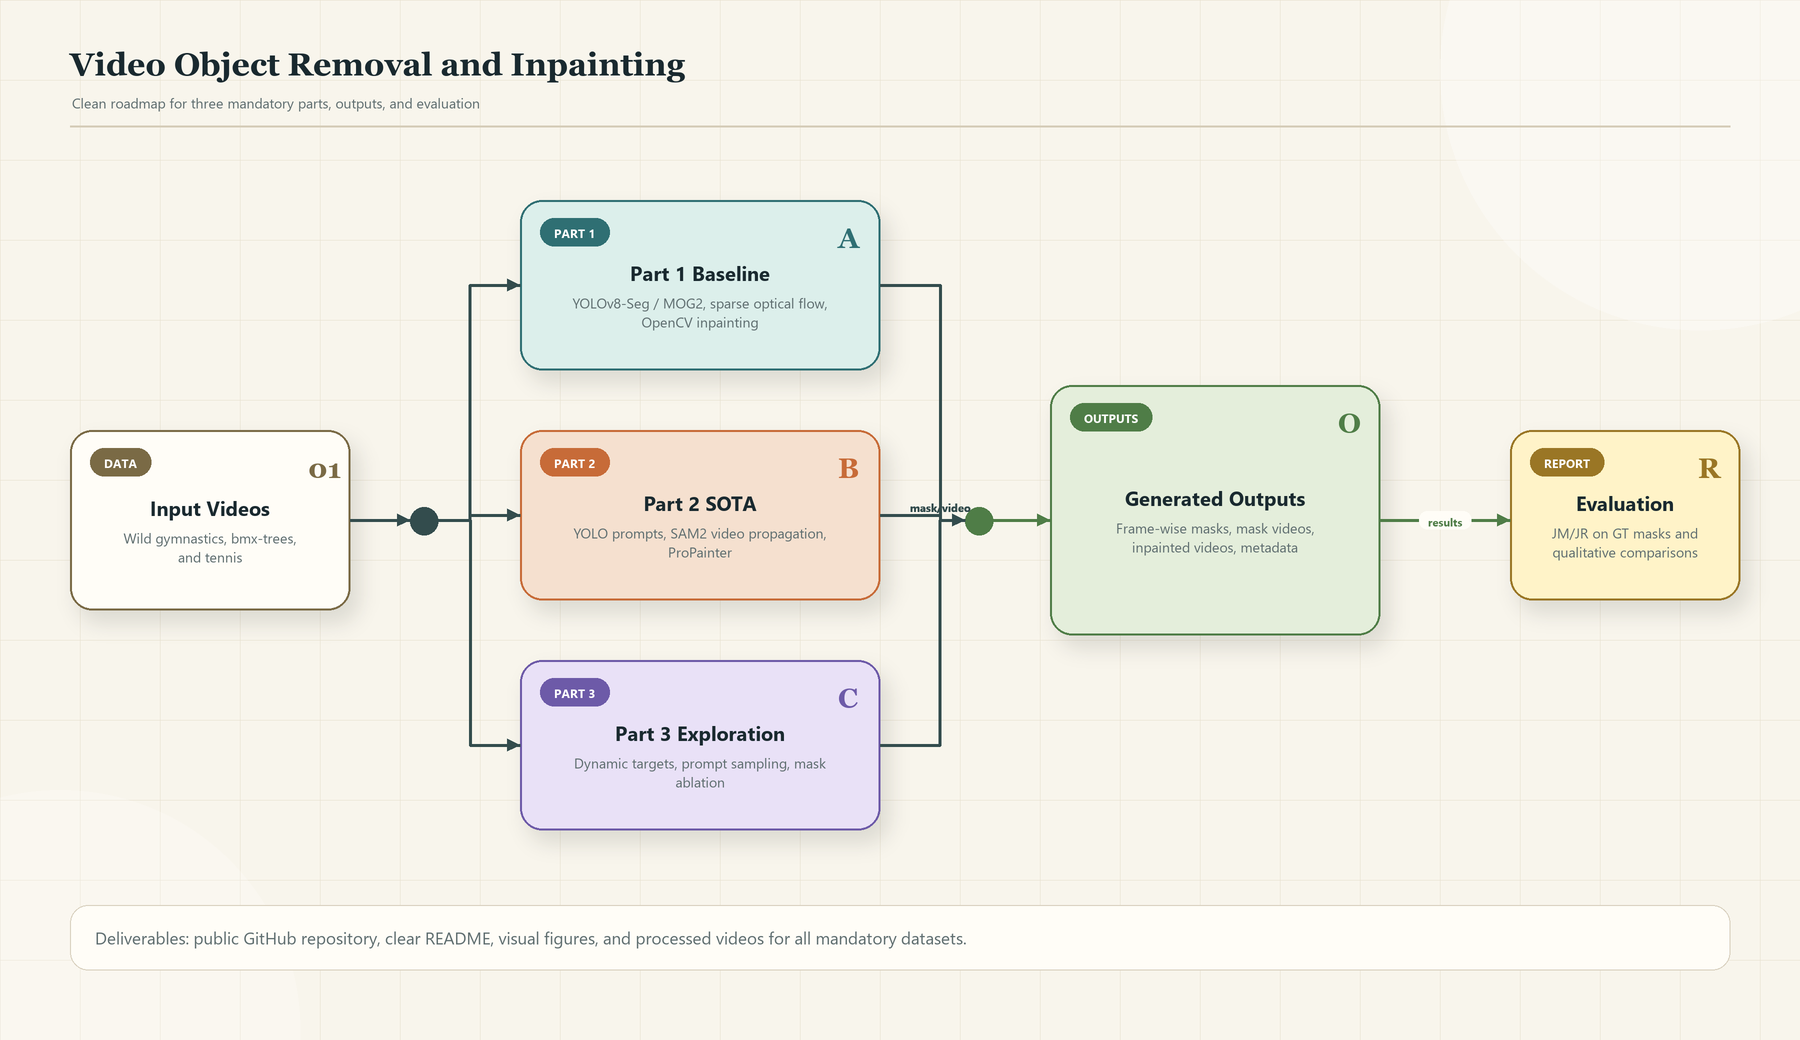
\includegraphics[width=0.93\textwidth]{flowchart_overview.png}
    \caption{Overall roadmap. Part 1 provides an interpretable baseline, Part 2 is the main SAM2 + ProPainter pipeline, and Part 3 studies refinement and SAM3/DiffuEraser extensions.}
    \label{fig:overview}
\end{figure*}

\subsection{Part 1: Interpretable Baseline}
The Part 1 baseline is designed to be understandable and reproducible. It first estimates candidate foreground regions from object cues and motion differences. Because a single-frame mask can be noisy, the mask sequence is filtered temporally: small isolated components are removed, short gaps are filled, and masks are dilated only enough to cover uncertain boundaries. The final mask is passed to an OpenCV inpainting backend.

This baseline is intentionally not the strongest possible method. Its role is to provide a reference point for later improvements. It performs reasonably on simple human-motion cases, but its limitations are clear on bmx-trees, where the bicycle contains thin spokes and hollow wheels. A classical mask often becomes too solid or too fragmented, which lowers IoU against a detailed ground-truth mask. This weakness is useful in the report because it explains why Part 2 is necessary.

The main advantage of Part 1 is controllability. Each operation has an interpretable effect: dilation increases coverage, component filtering suppresses isolated noise, and temporal smoothing reduces frame-to-frame flicker. However, these rules are local and cannot understand object identity. If the target is partially occluded or temporarily changes pose, the baseline has no memory of the object beyond simple temporal heuristics. This is the central reason why Part 1 is kept as a baseline rather than the final method.

\subsection{Part 2: SAM2 + ProPainter}
Part 2 is our main final pipeline. It begins with target localization, then converts the target into prompts for SAM2. SAM2 propagates the mask over the video and produces a temporally coherent binary mask sequence. We then apply mask dilation and consistency checks to reduce boundary leakage before passing the frames and masks to ProPainter.

The advantage of this design is that segmentation and inpainting are matched to their strengths. SAM2 is strong at tracking an object through appearance changes, while ProPainter is strong at filling the removed area in a video-aware manner. In practice, this combination substantially improves \jm\ and \jr\ on the mandatory sample videos and on the full DAVIS evaluation. It also produces more visually stable inpainted videos than the Part 1 OpenCV backend.

We also add engineering choices that matter in practice. The pipeline supports low-memory ProPainter settings for long or high-resolution videos, keeps mask and inpainting outputs in separate folders, and stores the final configuration with each run. This is important because video inpainting results are sensitive to resolution, mask dilation, and temporal window length. By making these settings explicit, the experiments are reproducible rather than being one-off demos.

\subsection{Part 3: Refinement and Exploration}
Part 3 contains two complementary branches. Part 3A is an adaptive refinement module placed after SAM2 propagation. It uses optical-flow magnitude and temporal mask statistics to suppress static false positives and recover moving object regions. This is particularly helpful when SAM2 over-segments background regions or when the object undergoes fast non-rigid motion. The breakdance experiment is our strongest evidence for this branch.

Part 3B is a secondary exploration branch using SAM3 and DiffuEraser or ProPainter. We keep it as an ablation rather than replacing Part 2. The reason is empirical: SAM3 completes more DAVIS sequences but does not improve the average DAVIS \jm/\jr. This makes Part 3B valuable as a robustness and failure-mode study rather than a universal final solution.

The two Part 3 branches answer different questions. The adaptive branch asks whether a strong Part 2 mask can be improved by using motion and temporal consistency after propagation. The SAM3 branch asks whether replacing the segmentation backbone changes the overall behavior. Keeping both branches in the report gives a stronger experimental narrative: Part 3 is not a disconnected extra feature, but a controlled study of how to improve or stress-test the Part 2 pipeline.

\subsection{Target Definition and Mask Post-processing}
A subtle but important issue in object removal is the definition of the target itself. In some sequences, the target is a single person; in others, the semantic target includes the object being manipulated, such as a bicycle or racket. We therefore treat the target as the visually coherent foreground action rather than only the human body. This choice is especially important for bmx-trees: removing only the rider while leaving the bicycle would not satisfy the visual goal of removing the moving foreground event. At the same time, the GT mask may preserve hollow structures such as bicycle wheels, so an overly solid mask can lower IoU even if it removes the correct object visually.

To balance mask coverage and geometric precision, we use conservative post-processing instead of uniform aggressive dilation. Small connected components are removed when they are inconsistent with the target location, while boundary dilation is used only to cover uncertain object edges that would otherwise leave ghost artifacts after inpainting. In Part 3, motion cues are used as an additional filter: regions that remain static across frames are less likely to be part of the moving target and can be suppressed. This post-processing policy connects the metric goal and the visual goal. It avoids optimizing IoU alone at the cost of visible residuals, and it also avoids masking a very large area that would make the inpainting task unnecessarily difficult.


\section{Implementation Details}
The implementation is organized as a set of command-line pipelines rather than notebook-only experiments. This is important for reproducibility because each processed video can be regenerated from an input path, a configuration file, and a selected backend. The main scripts are \texttt{part1\_pipeline.py}, \texttt{part2\_pipeline.py}, \texttt{part3\_pipeline.py}, \texttt{part23\_integrated\_pipeline.py}, and \texttt{part3\_sam3\_pipeline.py}. Intermediate results are saved explicitly, including frames, masks, overlays, restored frames, final videos, and configuration summaries. This file structure lets us inspect whether an error comes from segmentation, mask post-processing, or inpainting.

For Part 2, the implementation uses adapter scripts for external models. This avoids mixing project logic with third-party inference code. The SAM2 adapter is responsible for mask propagation, while the ProPainter adapter is responsible for video completion. The pipeline can also run low-memory settings for longer videos by lowering resolution or changing temporal window parameters. These settings were important for DAVIS and wild-video experiments because a single high-resolution video may otherwise exceed GPU memory.

For Part 3, the integrated runner supports different refinement modes. The default Part 2 mode preserves the original SAM2 mask as much as possible. The motion-strict mode suppresses regions that are inconsistent with foreground motion, and the adaptive mode combines motion cues with temporal recovery. This design makes ablation straightforward: we can compare raw SAM2, motion filtering, and final adaptive refinement on the same input video and with the same evaluation script. The SAM3 branch is kept separate but follows the same naming convention, so its outputs can be compared with Part 2 and Part 3A results.

Table~\ref{tab:impl_summary} summarizes the final runnable components. We include this table because the project is not only a set of reported numbers; it is also expected to be reproducible from submitted code and processed outputs.

\begin{table*}[t]
\centering
\caption{Implementation summary of the final pipelines. Script names are line-broken only for layout; the submitted repository keeps the full filenames. Each part saves intermediate masks and final videos so that mask errors and inpainting errors can be inspected separately.}
\label{tab:impl_summary}
\small
\resizebox{0.96\textwidth}{!}{%
\begin{tabular}{p{0.10\textwidth}p{0.18\textwidth}p{0.24\textwidth}p{0.18\textwidth}p{0.20\textwidth}}
\toprule
\textbf{Part} & \textbf{Main script} & \textbf{Mask source} & \textbf{Inpainting backend} & \textbf{Main outputs} \\
\midrule
Part 1 & \begin{tabular}[t]{@{}l@{}}\texttt{part1}\texttt{\_pipeline.py}\end{tabular} & Classical object and motion cues with temporal smoothing & OpenCV frame-level inpainting & masks, overlays, baseline restored video \\
Part 2 & \begin{tabular}[t]{@{}l@{}}\texttt{part2}\texttt{\_pipeline.py}\end{tabular} & Prompted SAM2 video propagation with conservative post-processing & ProPainter video inpainting & propagated masks, ProPainter result, final video \\
Part 3A & \begin{tabular}[t]{@{}l@{}}\texttt{part3}\texttt{\_pipeline.py}\\\texttt{part23}\texttt{\_integrated}\\\texttt{\_pipeline.py}\end{tabular} & SAM2 masks refined by motion filtering and temporal recovery & ProPainter or inherited Part 2 backend & ablation masks, refined masks, difficult-case videos \\
Part 3B & \begin{tabular}[t]{@{}l@{}}\texttt{part3}\texttt{\_sam3}\\\texttt{\_pipeline.py}\end{tabular} & SAM3-based target segmentation branch & ProPainter or DiffuEraser & SAM3 ablation metrics and qualitative outputs \\
\bottomrule
\end{tabular}%
}
\end{table*}
\section{Evaluation Protocol}
For videos with ground-truth masks, we use frame-level IoU, following the DAVIS evaluation protocol and the JM/JR reporting style used by recent dynamic-scene segmentation work such as VGGT4D \cite{davis,vggt4d}:
\begin{equation}
\mathrm{IoU}_t = \frac{|M_t \cap G_t|}{|M_t \cup G_t|},
\end{equation}
where $M_t$ is the predicted mask and $G_t$ is the ground-truth mask at frame $t$. We report the mean IoU, denoted as \jm, and the recall-style IoU consistency score, denoted as \jr. Higher values indicate better masks.

For video quality, PSNR and SSIM require a clean target-free video as ground truth. The mandatory bmx-trees, tennis, and wild gymnastics videos do not provide such target-free references. Therefore, we submit the processed videos and use qualitative visual comparisons for inpainting quality, which follows the course update for datasets without ground truth. DAVIS experiments are used primarily for mask-quality evaluation because DAVIS provides segmentation masks.

Our qualitative evaluation focuses on three visible properties. First, the removed object should not leave a strong silhouette or boundary artifact. Second, the restored background should remain temporally stable rather than flickering between frames. Third, the result should not remove unrelated objects unless they are part of the target interaction. These criteria are used when discussing the mandatory videos and the wild video, where pixel-level target-free references are unavailable.

Table~\ref{tab:eval_setting} summarizes how each dataset is used. This table is included to make the evaluation policy explicit: mask metrics are reported when GT masks are available, while restored-video quality is judged qualitatively when no clean target-free video exists.

\begin{table*}[t]
\centering
\caption{Dataset usage, available ground truth, and reported evidence. The setting follows the project update: quantitative video metrics are not required when clean target-free videos are unavailable.}
\label{tab:eval_setting}
\resizebox{0.96\textwidth}{!}{%
\begin{tabular}{p{0.16\textwidth}p{0.22\textwidth}p{0.17\textwidth}p{0.21\textwidth}p{0.16\textwidth}}
\toprule
\textbf{Dataset group} & \textbf{Videos / sequences} & \textbf{GT available} & \textbf{Reported evidence} & \textbf{Deliverable} \\
\midrule
Mandatory sample & bmx-trees, tennis & GT masks for mask evaluation; no clean target-free video & \jm/\jr\ for masks; qualitative restored-frame comparison & Processed videos and masks \\
Wild video & gymnastics video & No GT mask and no clean target-free video & Qualitative generalization analysis & Processed video \\
DAVIS full set & 50 DAVIS sequences & GT masks & Aggregate \jm/\jr\ and success/failure analysis & Metrics summary \\
DAVIS stress cases & walking, bike-packing, breakdance & GT masks & Per-case \jm/\jr\ plus failure-mode discussion & Metrics and visual comparison \\
Part 3 ablations & breakdance and SAM3/DiffuEraser runs & GT masks for DAVIS cases & Refinement ablation and backbone comparison & Tables and supplementary visuals \\
\bottomrule
\end{tabular}%
}
\end{table*}

\section{Experiments}
\subsection{Mandatory Sample Videos}
Table~\ref{tab:mandatory} shows the mandatory sample results. The final optimized setting improves both Part 1 and Part 2 over earlier settings. Part 2 achieves the strongest final scores on both bmx-trees and tennis. The tennis result is especially strong, with \jm\ increasing to 0.9342 and \jr\ reaching 1.0000.

\begin{table*}[t]
\centering
\caption{Mandatory sample mask metrics. Higher is better.}
\label{tab:mandatory}
\resizebox{0.96\textwidth}{!}{%
\begin{tabular}{llcccccc}
\toprule
\textbf{Dataset} & \textbf{Method} & \textbf{Initial \jm} & \textbf{Initial \jr} & \textbf{Final \jm} & \textbf{Final \jr} & \textbf{$\Delta$\jm} & \textbf{$\Delta$\jr} \\
\midrule
bmx-trees & Part 1 & 0.3557 & 0.2750 & 0.4098 & 0.4000 & +0.0541 & +0.1250 \\
bmx-trees & Part 2 & 0.5056 & 0.7000 & 0.6526 & 0.9250 & +0.1470 & +0.2250 \\
tennis & Part 1 & 0.6455 & 0.9857 & 0.7822 & 1.0000 & +0.1367 & +0.0143 \\
tennis & Part 2 & 0.7127 & 1.0000 & 0.9342 & 1.0000 & +0.2214 & +0.0000 \\
\bottomrule
\end{tabular}%
}
\end{table*}

The lower bmx-trees score is expected because the object includes a rider and bicycle. The ground-truth bicycle wheels are hollow, while automatic masks tend to fill the wheel interiors. This difference hurts IoU even when the visual removal looks reasonable. We therefore interpret bmx-trees as a strict mask-geometry test, not only an inpainting-quality test.

The tennis sequence is easier from the mask-geometry perspective because the target occupies a more compact region and has fewer internal holes. This explains why both Part 1 and Part 2 achieve high \jr, while Part 2 still improves the mean IoU substantially. In the final video, the difference is also visible: the SAM2 mask is more stable around the moving player, and ProPainter produces fewer frame-wise artifacts than the OpenCV baseline.

\begin{figure*}[t]
    \centering
    \begin{subfigure}{0.49\textwidth}
        \centering
        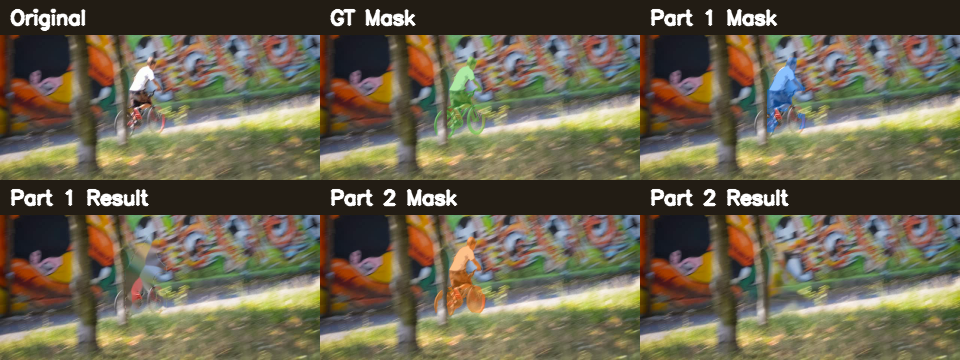
\includegraphics[width=\textwidth]{part12_improved_final_bmx_comparison.png}
        \caption{bmx-trees}
    \end{subfigure}
    \hfill
    \begin{subfigure}{0.49\textwidth}
        \centering
        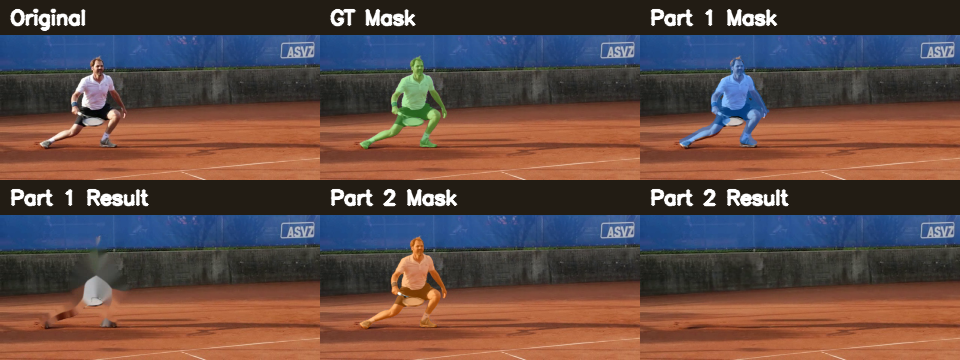
\includegraphics[width=\textwidth]{part12_improved_final_tennis_comparison.png}
        \caption{tennis}
    \end{subfigure}
    \caption{Qualitative comparison on mandatory sample videos. The visual results complement the mask metrics in Table~\ref{tab:mandatory}.}
    \label{fig:mandatory_vis}
\end{figure*}

\subsection{Wild Video}
The wild gymnastics video is used for generalization. Since it has no ground-truth mask or clean target-free video, we do not report \jm/\jr, PSNR, or SSIM. Instead, the processed videos are submitted and evaluated qualitatively. In the final outputs, the mask is sufficiently stable for most of the motion, and the restored video is useful as a real-world demonstration. A representative qualitative figure is placed in the appendix to keep the main paper within the target length.

\subsection{Full DAVIS Evaluation}
To avoid overfitting the report to the mandatory examples, we also ran Part 1 and Part 2 on the full DAVIS 50-sequence set. Table~\ref{tab:davis} summarizes the result. Part 2 succeeds on 48 sequences and reaches 0.7429 mean \jm, while Part 1 succeeds on 37 sequences and reaches 0.5334 mean \jm. On the 35 sequences where both methods succeed, Part 2 improves mean \jm\ by +0.1706 and mean \jr\ by +0.1757.

\begin{table}[t]
\centering
\caption{Full DAVIS 50-sequence evaluation.}
\label{tab:davis}
\resizebox{\columnwidth}{!}{%
\begin{tabular}{lcccc}
\toprule
\textbf{Method} & \textbf{Succ.} & \textbf{Fail/Skip} & \textbf{Mean \jm} & \textbf{Mean \jr} \\
\midrule
Part 1 baseline & 37 & 13 & 0.5334 & 0.6072 \\
Part 2 SAM2+ProPainter & 48 & 2 & 0.7429 & 0.8239 \\
\bottomrule
\end{tabular}%
}
\end{table}

The DAVIS result is important because it confirms that Part 2 is not merely tuned to bmx-trees and tennis. Large improvements occur on dog-agility, horsejump-high, horsejump-low, dance-twirl, and hike. The remaining failures, including kite-surf and kite-walk, are useful limitations: they involve difficult appearance changes, background ambiguity, or target definitions that are hard to express with a single automatic prompt.

The success-rate difference is also meaningful. Part 1 skips or fails more sequences because it depends on category-specific and motion-specific assumptions. Part 2 fails less often because SAM2 can propagate a prompted object beyond the initial detection. This is why the full DAVIS result is stronger evidence than a single cherry-picked example: it measures both average mask quality and operational robustness across many visual conditions.

\subsection{Failure Taxonomy}
Beyond aggregate scores, we also inspected the dominant failure modes of the current system. The most important errors are thin or hollow structures, fast non-rigid motion, intermittent visibility, background ambiguity, and inpainting residuals. These observations explain why our final method does not rely on a single universal post-processing rule: thin structures require conservative masks, while fast motion and background ambiguity benefit from motion-guided refinement. A detailed failure taxonomy with symptoms, causes, and design responses is provided in Appendix~\ref{app:failure_taxonomy}.

This analysis is important for interpreting the metrics. For example, a filled bicycle wheel can reduce IoU against a hollow ground-truth mask, but it may still remove the foreground object visually. Conversely, a mask with acceptable mean IoU can still produce visible artifacts if a few frames are temporally inconsistent. Therefore, our final evaluation combines numerical evidence with frame-level visual inspection.
\subsection{Part 3 Ablation and Difficult Cases}
Table~\ref{tab:part3} combines the most important Part 3 evidence. On breakdance, raw Part 2 produces a low mask score because the target is fast and non-rigid. Motion-strict refinement improves the score, and the full adaptive refinement reaches 0.6332 \jm\ and 0.8690 \jr. This is the clearest case where Part 3 improves over Part 2. Figure~\ref{fig:main_ablation} visualizes the ablation behavior, while the larger final qualitative comparison is kept in Supplementary Fig.~\ref{fig:supp_qualitative}.

\begin{table}[!t]
\centering
\caption{Compact Part 3 evidence. The first block shows the breakdance refinement gain; the second block summarizes the full-DAVIS SAM3 branch.}
\label{tab:part3}
\resizebox{\columnwidth}{!}{%
\begin{tabular}{llcc}
\toprule
\textbf{Group} & \textbf{Method} & \textbf{\jm} & \textbf{\jr} \\
\midrule
breakdance & Part 1 & 0.1529 & 0.0000 \\
breakdance & Part 2 & 0.3453 & 0.0000 \\
breakdance & motion strict & 0.4740 & 0.7500 \\
breakdance & Part 3 adaptive & 0.6332 & 0.8690 \\
\midrule
DAVIS & SAM2 + DiffuEraser & 0.7429 & 0.8239 \\
DAVIS & SAM3 + DiffuEraser & 0.6839 & 0.7410 \\
DAVIS & SAM3 + ProPainter & 0.6839 & 0.7410 \\
\bottomrule
\end{tabular}%
}
\end{table}
\begin{figure*}[!t]
    \centering
    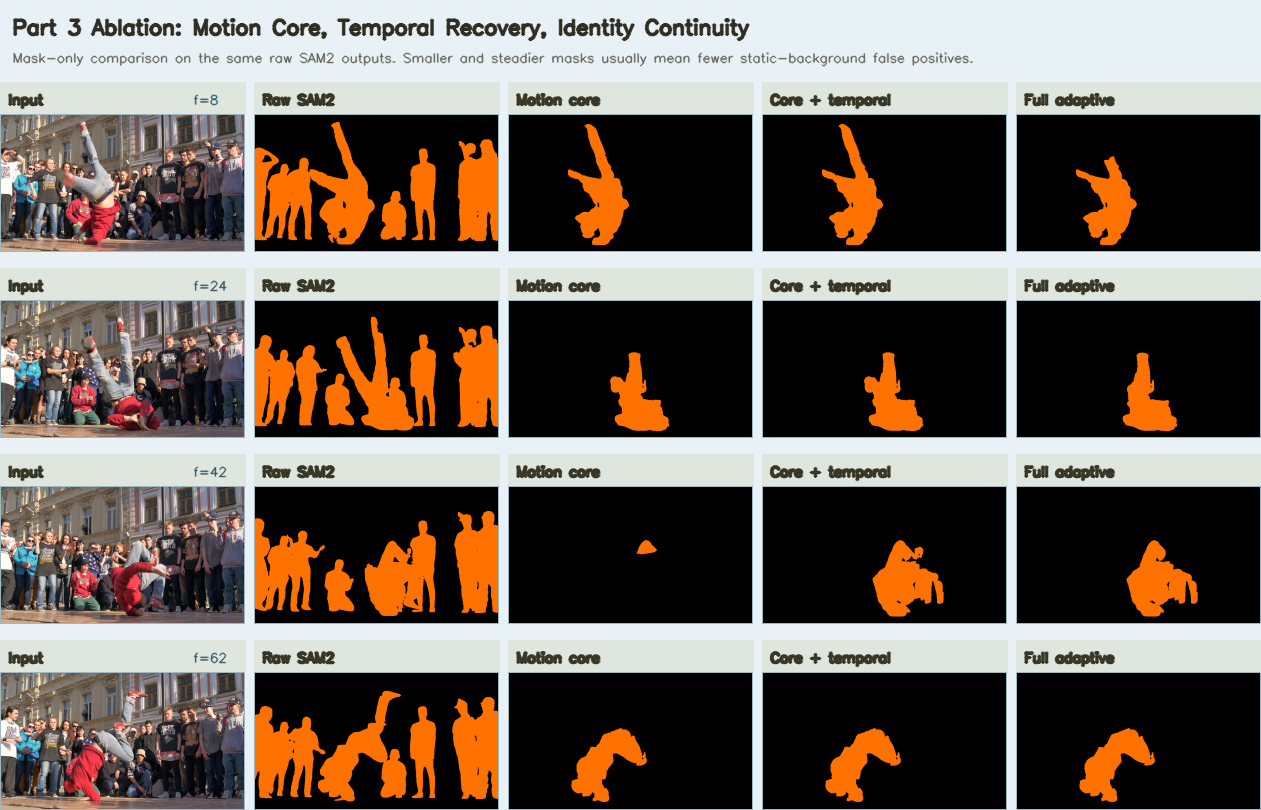
\includegraphics[width=0.72\textwidth]{part3_breakdance_ablation.png}
    \vspace{-0.4em}
    \caption{Main-paper Part 3 ablation visualization on breakdance. Raw SAM2 masks over-segment the dynamic scene, motion filtering suppresses many false positives, and temporal recovery improves object continuity. This figure complements the quantitative gains in Table~\ref{tab:part3}.}
    \label{fig:main_ablation}
    \vspace{-0.6em}
\end{figure*}

The SAM3 branch gives a more nuanced result. It completes all 50 DAVIS sequences, which is useful from a robustness perspective, but it is not the best average mask-quality solution. On common successful sequences, SAM3 improves some categories such as motorbike, train, soccerball, stroller, and tennis, but drops on rhino, dance-twirl, dance-jump, goat, and hike. We therefore present it as a meaningful exploration rather than the final replacement for Part 2.

This conclusion is useful for a high-quality project because it avoids overfitting the story to a single positive result. A less rigorous presentation might only show the cases where SAM3 is better. Instead, our ablation shows both gains and drops, then explains how the evidence should be interpreted. The final recommendation is to use Part 2 as the default method, apply Part 3 adaptive refinement for hard motion cases, and treat SAM3 as a candidate branch that needs per-video validation.

\FloatBarrier
\section{Discussion}
The experiments support three conclusions. First, Part 1 is valuable as a transparent baseline, but it is not sufficient for high-quality video object removal. Its masks are sensitive to thin structures and complex motion, and its frame-wise inpainting cannot guarantee temporal consistency. Second, Part 2 is the strongest general-purpose pipeline in our submission. It improves the mandatory metrics and performs well on the full DAVIS evaluation. Third, Part 3 is useful when framed as targeted refinement and ablation. The adaptive branch clearly improves a difficult case, while the SAM3 branch reveals both benefits and trade-offs.

The main limitation is that inpainting quality cannot be fully summarized by \jm\ and \jr. These metrics evaluate masks, not texture realism. For mandatory videos without clean target-free backgrounds, qualitative evaluation remains necessary. Another limitation is object definition. In bmx-trees, whether the wheel interior should be empty or filled has a large effect on IoU. Human-object interaction therefore needs careful mask conventions.

Future work should focus on adaptive target definitions and better uncertainty handling. One direction is to learn when to preserve holes and thin structures instead of applying uniform dilation. Another direction is to select between SAM2, SAM3, and motion refinement automatically based on video properties. Finally, a stronger report could include user studies or perceptual metrics for inpainting quality when clean background ground truth is unavailable.

In terms of deployment, the most important next step would be an automatic quality-control module. Such a module could compare mask area variation, optical-flow consistency, and detection confidence to decide whether the default Part 2 output is reliable. If the indicators suggest over-segmentation or temporal drift, the system could switch to the Part 3 adaptive branch automatically. This would turn the current experimental insight into a more practical end-to-end object-removal tool.

A second future direction is to make target definition interactive. In real applications, the user may want to remove only a person, a person plus an object, or a complete activity region. The current system uses automatic assumptions that work well for the assignment, but a lightweight user confirmation step could resolve ambiguous cases such as rider-only versus rider-plus-bicycle removal. This would likely improve both visual satisfaction and metric alignment, because the predicted mask would better match the intended target convention.

Finally, future evaluation could include perceptual video metrics or human preference studies for inpainting quality. Mask IoU measures whether the correct pixels were selected for removal, but it does not measure whether the synthesized background is believable. A complete evaluation protocol for object removal should therefore combine mask accuracy, temporal stability, and perceptual realism.

\section{Conclusion}
We completed all three required parts of the project. Part 1 provides an interpretable baseline, Part 2 gives the strongest overall system with SAM2 and ProPainter, and Part 3 adds meaningful refinement and SAM3/DiffuEraser exploration. Quantitative results are reported whenever ground-truth masks are available, and qualitative comparisons are used for mandatory videos without clean target videos. The final evidence shows that the project is complete, experimentally supported, and suitable for submission.

The main limitation is that the project still depends on accurate target definition. In sequences such as bmx-trees, the expected mask may include hollow wheel structures, while automatic object-removal masks tend to become more solid for safer inpainting. This creates a real trade-off between metric alignment and visual removal quality. Another limitation is that PSNR and SSIM cannot be computed for mandatory videos without clean target-free reference videos, so qualitative judgment remains necessary for restored-video realism.

Future work should make this decision process more adaptive. A stronger system could automatically choose between the default Part 2 pipeline, motion-strict filtering, adaptive Part 3 refinement, and SAM3-based prompts according to mask confidence, motion stability, and target ambiguity. This would turn the current experimentally validated modules into a more reliable end-to-end object-removal system.

\FloatBarrier
{\small
    \bibliographystyle{ieeenat_fullname}
    \bibliography{main}
}

\onecolumn
\appendix
\section{Supplementary Material}
This supplementary material contains supporting visual evidence for the main report. The main paper keeps only the most important quantitative tables and qualitative figures, while the supplementary pages preserve detailed roadmaps and additional visual comparisons for reproducibility. These figures should be read together with the main-paper metrics: they illustrate visual behavior but are not used as extra quantitative claims.

\begin{figure}[!htbp]
    \centering
    \begin{subfigure}{0.32\textwidth}
        \centering
        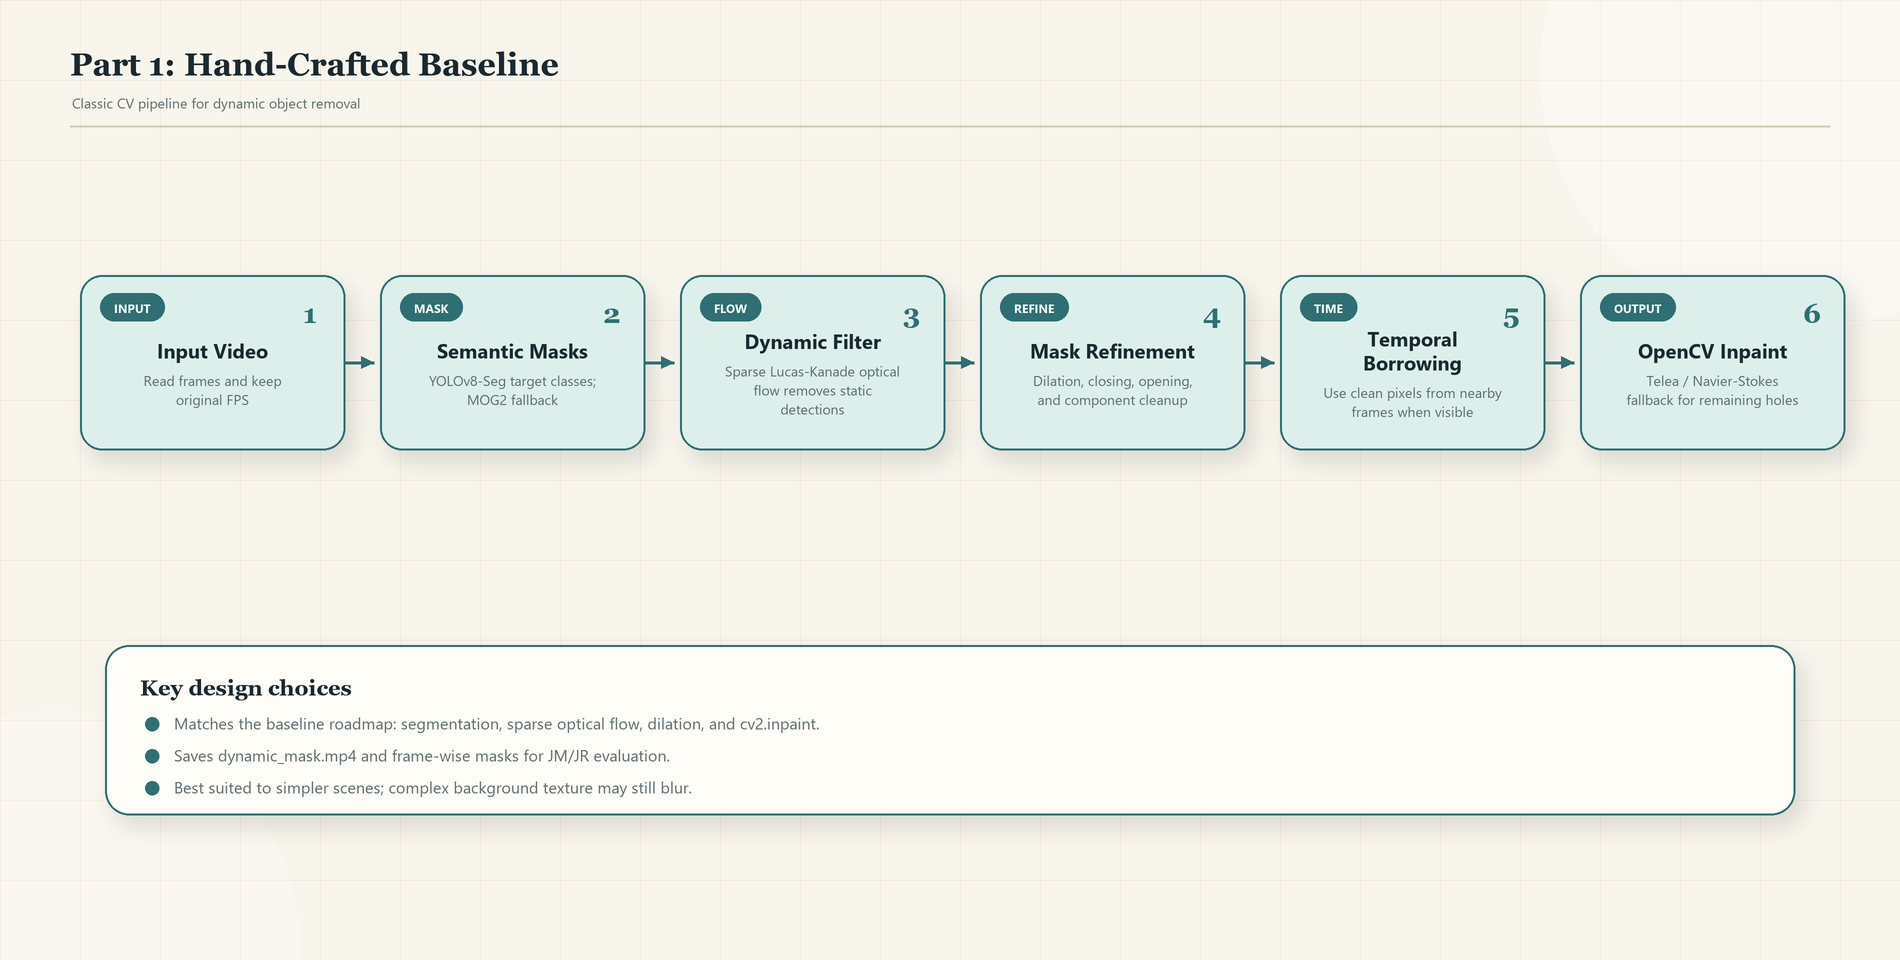
\includegraphics[width=\textwidth]{flowchart_part1.png}
        \caption{Part 1 baseline.}
    \end{subfigure}\hfill
    \begin{subfigure}{0.32\textwidth}
        \centering
        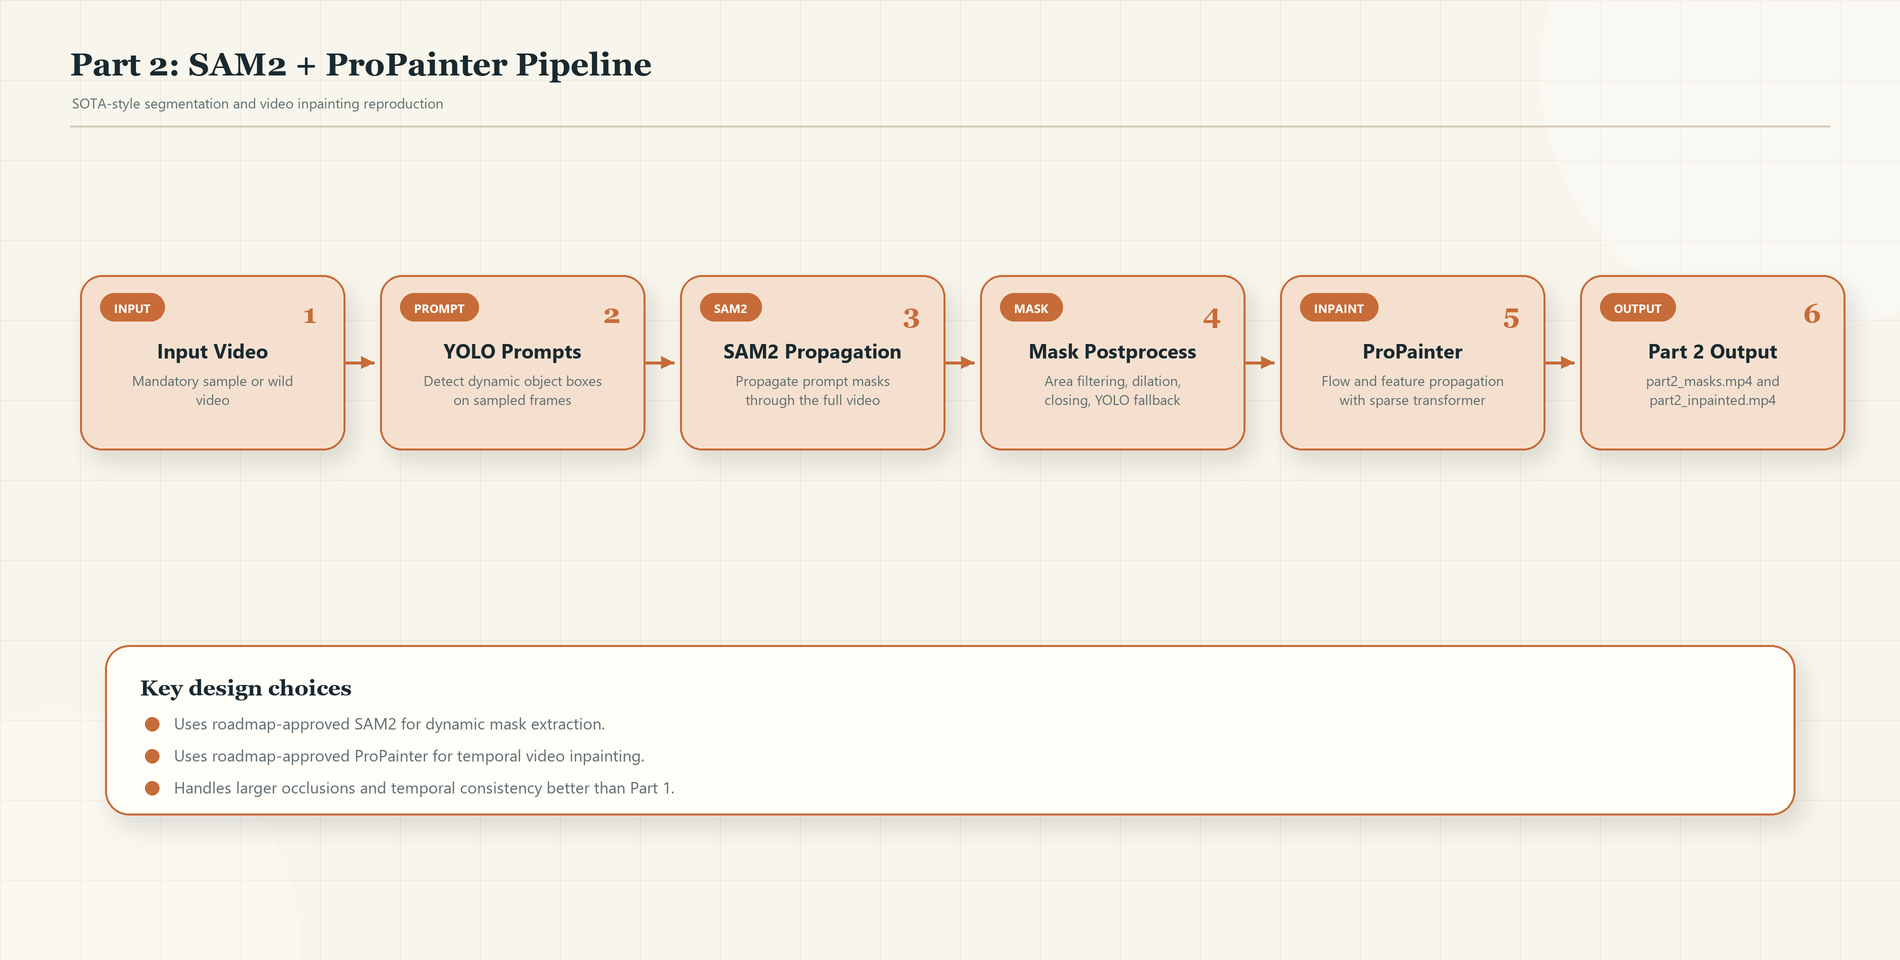
\includegraphics[width=\textwidth]{flowchart_part2.png}
        \caption{Part 2 SAM2 + ProPainter.}
    \end{subfigure}\hfill
    \begin{subfigure}{0.32\textwidth}
        \centering
        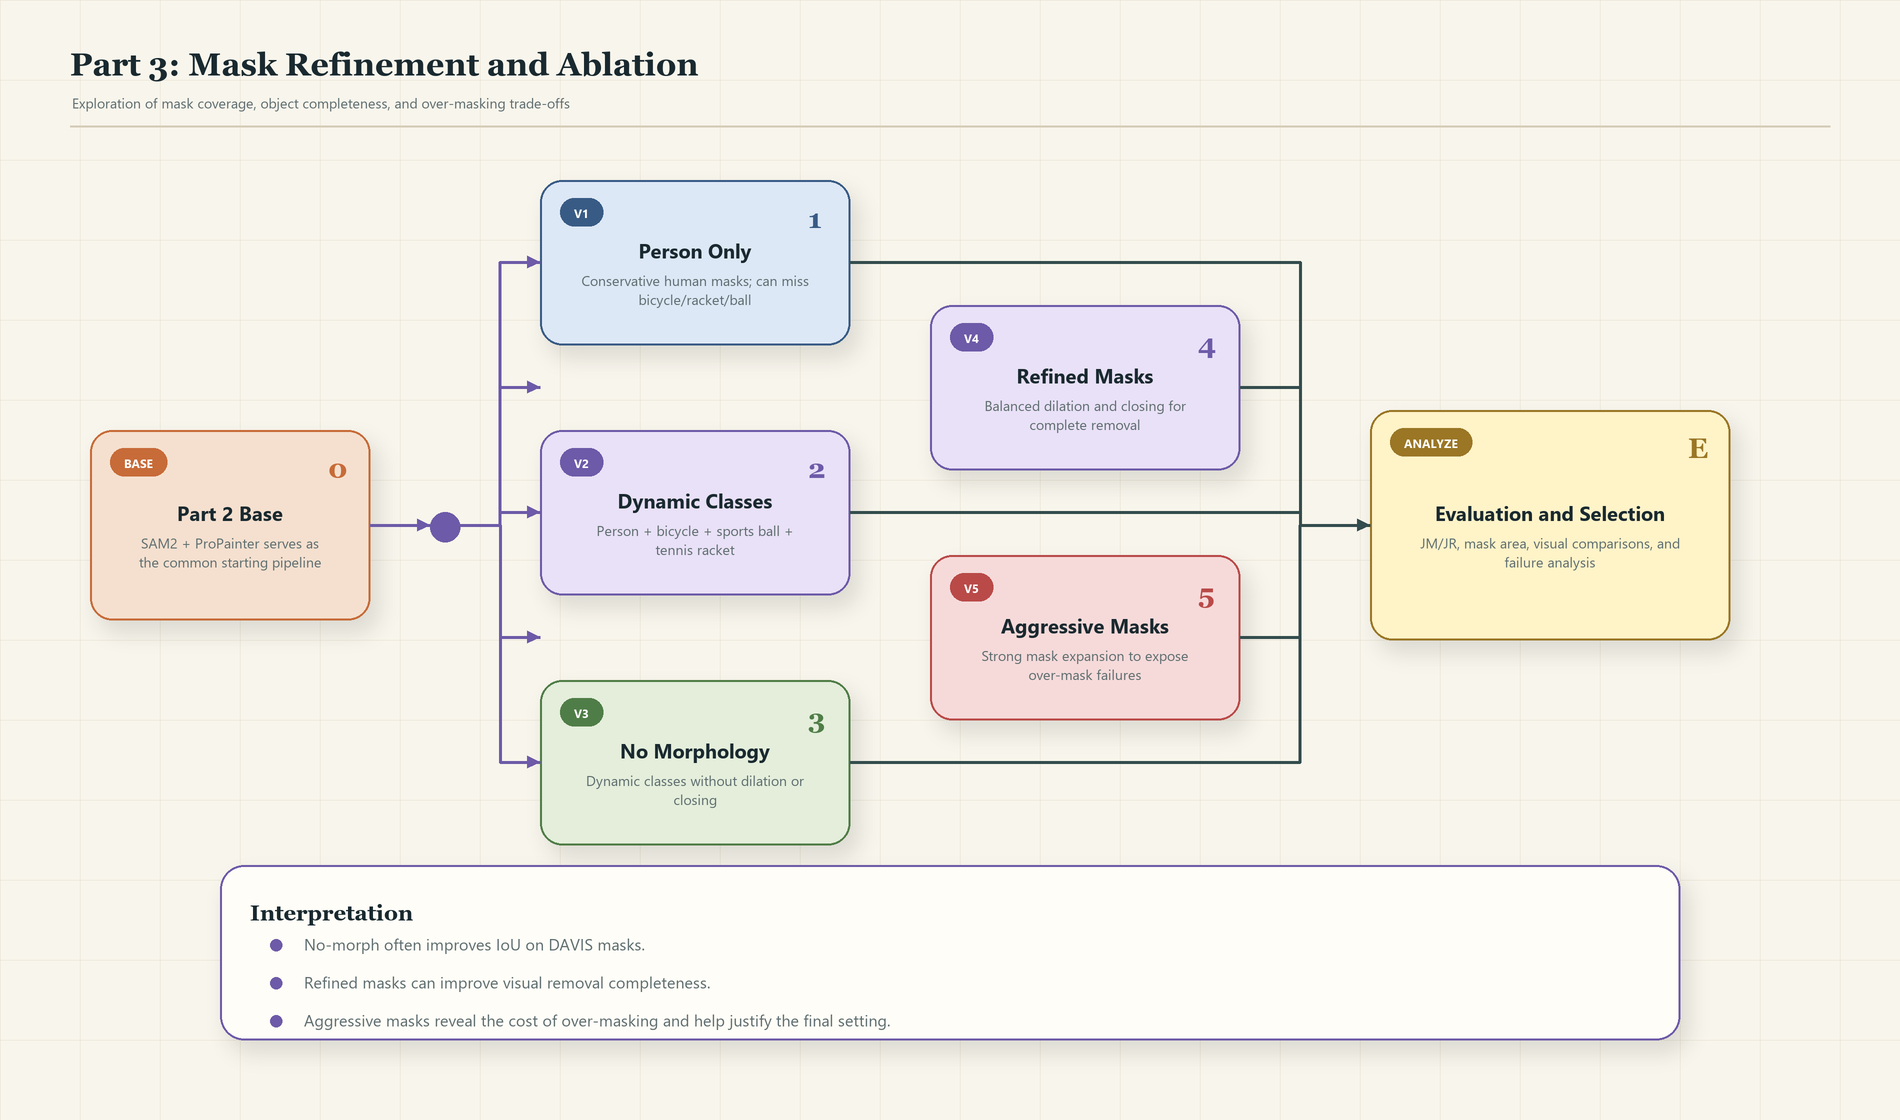
\includegraphics[width=\textwidth]{flowchart_part3.png}
        \caption{Part 3 refinement.}
    \end{subfigure}
    \vspace{-0.4em}
    \caption{Detailed technical roadmaps for the three required project parts. These diagrams expand the compact overview in the main paper and clarify the exact role of each module.}
    \label{fig:supp_flowcharts}
    \vspace{-0.8em}
\end{figure}

\begin{figure}[!htbp]
    \centering
    \begin{subfigure}{0.49\textwidth}
        \centering
        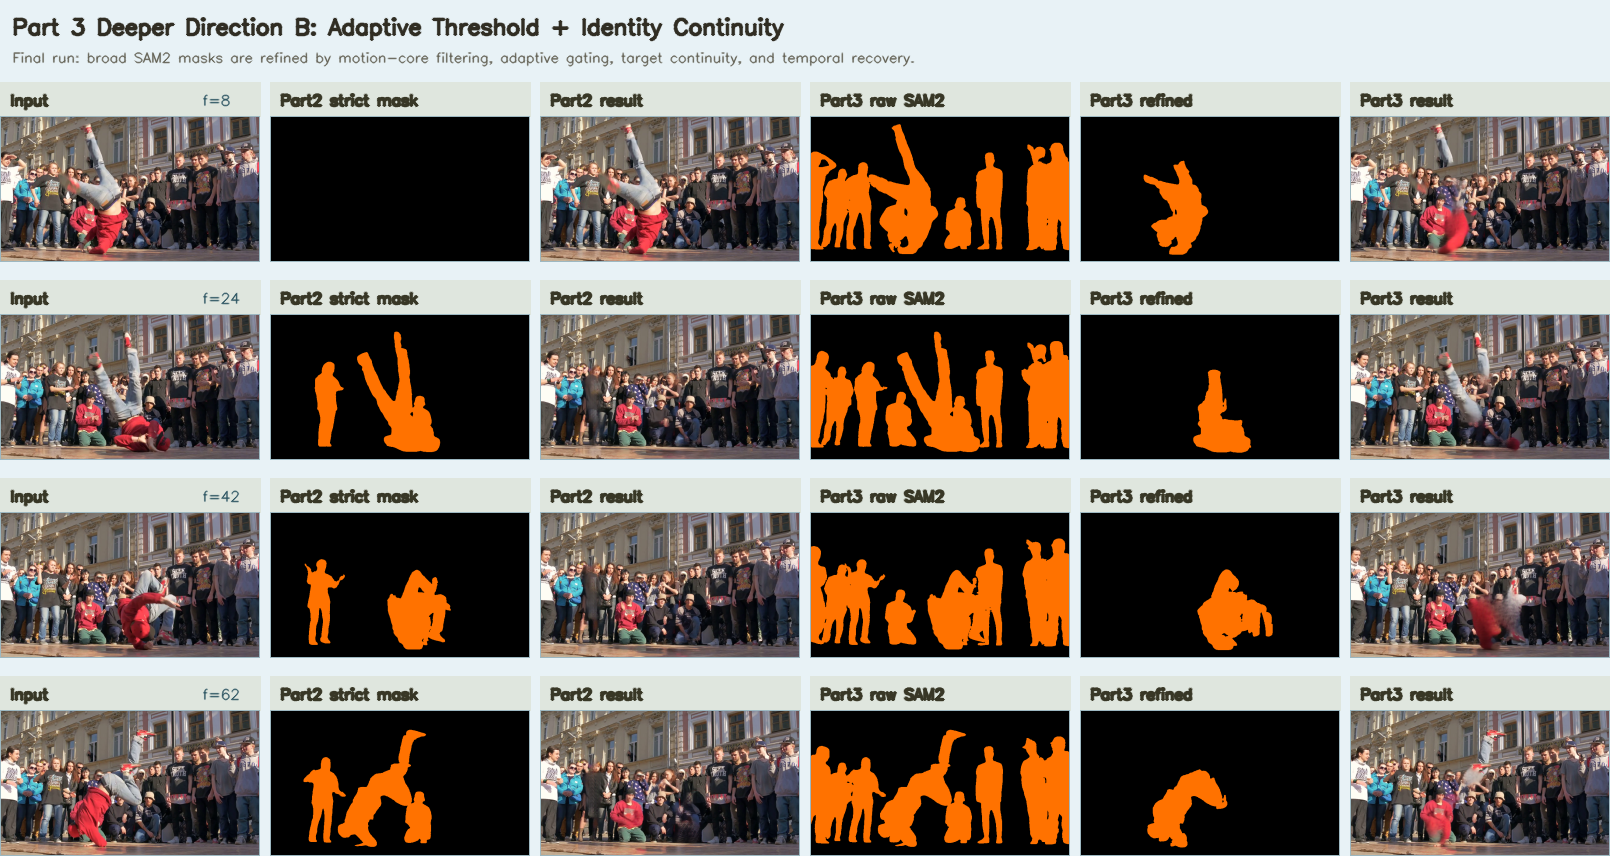
\includegraphics[width=\textwidth]{part3_breakdance_final_comparison.png}
        \caption{Final adaptive-refinement result on breakdance.}
    \end{subfigure}\hfill
    \begin{subfigure}{0.49\textwidth}
        \centering
        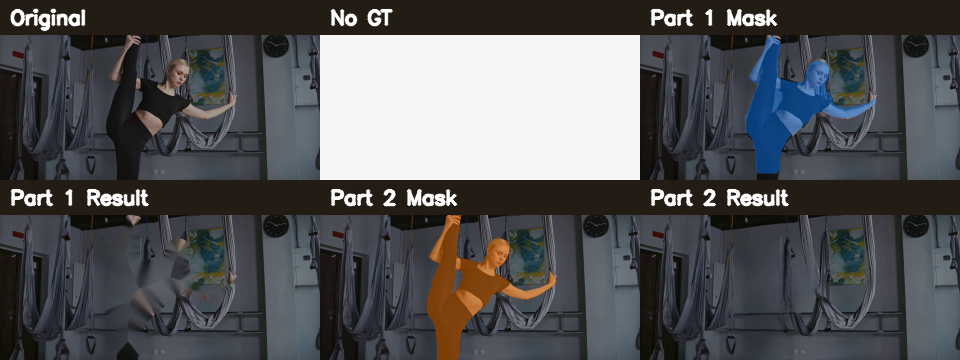
\includegraphics[width=\textwidth]{part12_improved_final_wild_gymnastics_comparison.png}
        \caption{Wild gymnastics qualitative result.}
    \end{subfigure}

    \vspace{0.35em}
    \begin{subfigure}{0.58\textwidth}
        \centering
        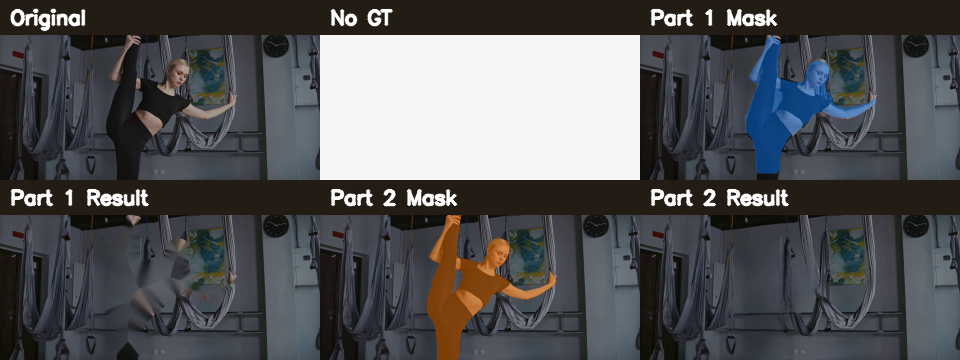
\includegraphics[width=\textwidth]{part3_sam3_wild_gymnastics_comparison.png}
        \caption{SAM3 branch qualitative output on the wild video.}
    \end{subfigure}
    \vspace{-0.4em}
    \caption{Supplementary qualitative evidence. The breakdance panel shows the final refined output for fast non-rigid motion, while the wild-video panels show generalization behavior on a non-DAVIS input without ground-truth masks.}
    \label{fig:supp_qualitative}
    \vspace{-0.8em}
\end{figure}


\section{Failure Taxonomy Details}
\label{app:failure_taxonomy}
This appendix expands the concise failure discussion in the main paper. The purpose of this taxonomy is not to introduce another metric, but to explain why different videos require different mask-refinement strategies. In video object removal, a visually plausible result depends on both where the mask is placed and how stable that mask remains over time. A method can obtain a reasonable average IoU while still producing visible flicker, or it can remove the target convincingly while receiving a lower IoU because the ground-truth mask uses a different structural convention.

\subsection{Motivation}
We built this taxonomy after inspecting the mandatory sample videos, the wild gymnastics video, and selected DAVIS stress cases. The inspection suggests that most remaining errors fall into five recurring categories: thin or hollow structures, fast non-rigid motion, intermittent visibility, background ambiguity, and inpainting residuals. These categories are useful because they connect visual failure cases to concrete design choices. For example, bicycle wheels expose the difference between a metric-oriented mask and an inpainting-oriented mask, while breakdance exposes the weakness of raw propagation under fast articulated motion.

\subsection{Detailed Categories}
Thin or hollow structures are most visible in bmx-trees. The ground-truth mask preserves wheel holes and thin spokes, but automatic masks often become more solid after propagation and dilation. This can reduce \jm even when the foreground object is removed visually. Fast non-rigid motion appears in breakdance-like sequences, where limbs and clothing change shape quickly and cause either missing regions or background leakage. Intermittent visibility is a temporal problem: when the target disappears or becomes weakly visible, a single initialization may not be enough to maintain identity. Background ambiguity happens when static objects resemble the target category or are close to the target region. Finally, inpainting residuals occur when the segmentation mask is too tight, leaving boundary pixels that ProPainter or OpenCV cannot fully remove.

\subsection{Design Implications}
The final system uses different responses for these different failure modes. Conservative dilation is used when structural precision matters, while a larger inpainting mask is used when boundary residues are visually harmful. Motion filtering is introduced for cases where static false positives dominate, and temporal recovery is used when a target briefly disappears. This is why the project does not report a single universal setting as optimal for every video. Instead, Part 2 is treated as the default high-quality pipeline, and Part 3 is used when motion or identity consistency becomes the limiting factor.

\begin{center}
\captionof{table}{Observed failure categories and the corresponding design response. The table connects qualitative error analysis with concrete method choices.}
\label{tab:failure_taxonomy_appendix}
\small
\resizebox{0.96\textwidth}{!}{%
\begin{tabular}{p{0.18\textwidth}p{0.24\textwidth}p{0.24\textwidth}p{0.22\textwidth}}
\toprule
\textbf{Failure type} & \textbf{Typical symptom} & \textbf{Likely cause} & \textbf{Design response} \\
\midrule
Thin or hollow structures & Bicycle wheels become filled or spokes disappear & Binary masks favor solid connected regions, while GT preserves internal holes & Use conservative dilation and report bmx-trees as a strict geometry case \\
Fast non-rigid motion & Mask misses limbs or includes nearby background & Appearance changes quickly and motion boundaries are unstable & Add Part 3 adaptive motion-guided refinement \\
Intermittent visibility & Object disappears and re-enters with weak propagation & The prompt is reliable only near the initial frames & Use temporal recovery and inspect overlay videos \\
Background ambiguity & Static background objects are included in the mask & Segmentation model confuses object-like background regions with the target & Apply motion filtering and connected-component consistency checks \\
Inpainting residuals & Removed region leaves a ghost outline & Mask boundary is too tight or temporally inconsistent & Use boundary-aware dilation and video-aware ProPainter completion \\
\bottomrule
\end{tabular}%
}
\end{center}

\subsection{Relation to Evaluation}
This taxonomy also clarifies why our evaluation combines quantitative and qualitative evidence. \jm and \jr are appropriate for measuring mask overlap when GT masks are available, but they do not directly measure whether the completed background looks natural. Conversely, a visually clean inpainting result may hide a mask that is too broad or structurally inconsistent with the GT annotation. The final report therefore treats DAVIS-style mask scores, mandatory-video qualitative comparisons, and ablation visualizations as complementary evidence rather than interchangeable measurements.
\end{document}










